%\item Interpretation of results
Although the results described above do not present clear evidence that the Reggio Approach is an effective early childhood program, there are some patterns that emerge and interesting results. 

% summary of main results 

We consider the possibility that it is possible that over time, the programs grew to share more features. Under this scenario, the Reggio Approach and the alternatives would become more similar reducing the estimated treatment effects of the Reggio Approach.\footnote{See \citet{Elango_Hojman_etal_2016_Early-Edu} for a discussion of considering the counterfactual in early childhood education evaluations.} 

There is evidence of policies mandating the provision of early childhood education and encouraging certain guidelines with the aim of improving quality.\footnote{See Appendix~\ref{sec:eceexperiences} for a detailed discussion of these policies.} However, exact information on the trajectory of the systems attended by the individuals in our sample is not published to the best of the authors' knowledge. In order to understand the exact evolution of the programs' administrative and pedagogical components over time, we wrote a survey to structure interviews with key individuals in the different school systems of Reggio Emilia, Parma, and Padova (see Appendix~\ref{sec:survey} for a full description of the survey and its implementation). We asked if the schools had aspects that are also present in the Reggio Approach schools, as well as details about their specific programs. These key aspects that make up the Reggio Approach were collected from published materials as well as confirmed by staff of the Reggio Approach. 

We present the similarities and differences between the different programs in Figures~\ref{fig:agg-admin} and~\ref{fig:agg-ped}. Using results from the structured interviews, we compute the number of administrative and pedagogical components that each program shares with the Reggio Approach by school type, city, and year. We examine 14 administrative components and 12 pedagogical components. Over time, many of the programs other than the state programs, adopt more features present in the Reggio Approach. This is especially true of the Parma municipal program when examining administrative components. The other programs do not adopt as many pedagogical components as they do administrative ones. Even though the Reggio Approach remained distinctive when considering the sum of its elements, many of the alternative schools evolved to include certain elements.

\begin{figure}[H]
\begin{center}
\begin{subfigure}[b]{0.55\textwidth}
	\caption{Number of Administrative Characteristics in Common with the Reggio Approach}\label{fig:agg-admin}
	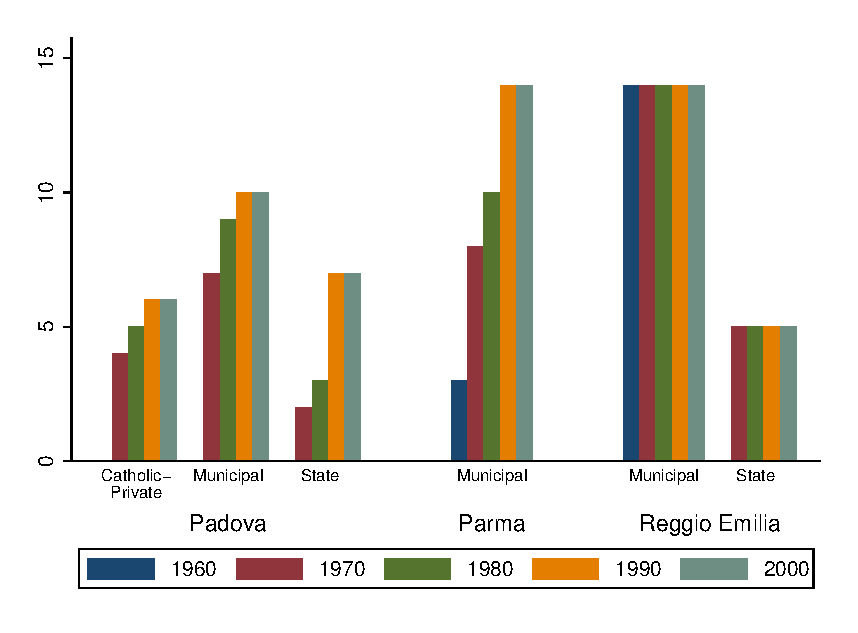
\includegraphics[width=\textwidth]{../../output/aggregateAdministrative.eps}
\end{subfigure}%
~
\begin{subfigure}[b]{0.55\textwidth}
	\caption{Number of Pedagogical Characteristics in Common with the Reggio Approach}\label{fig:agg-ped}
	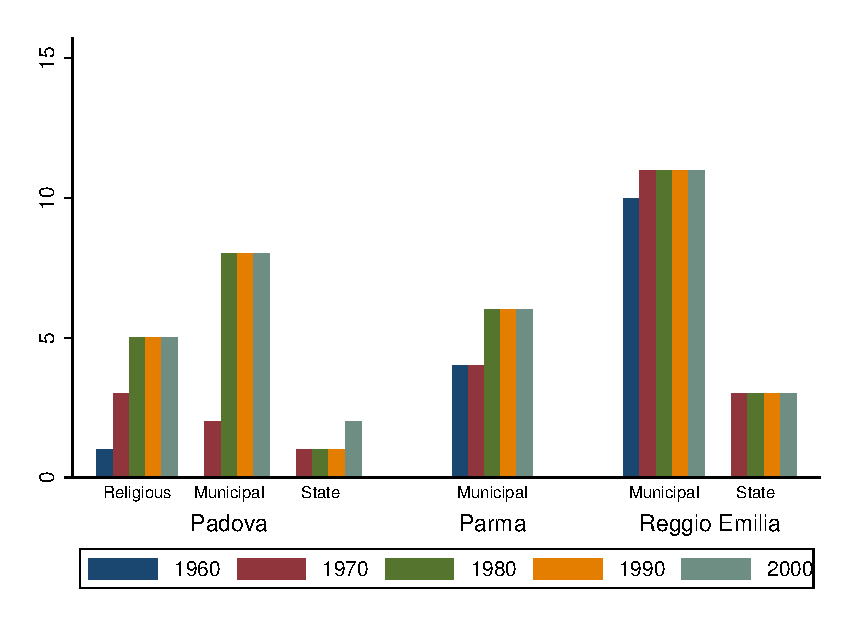
\includegraphics[width=\textwidth]{../../output/aggregatePedagogical.eps}
\end{subfigure}%
\end{center}
\raggedright \footnotesize Note: These graphs show the number of administrative and pedagogical components that each program has in common with the Reggio Approach. We consider 14 administrative components and 12 pedagogical components. One of the pedagogical components, following a set curriculum, was not present in the Reggio Approach. 
\end{figure}

% more details on survey results
The hours of center-based care is one commonality largely shared by the surveyed programs. All the programs except the state system in Padova offered additional hours for working families. Similarly, by the 1990s, all the surveyed systems received public funding. Some differences are seen in the teacher responsibilities. In the Reggio Approach, teachers have dedicated work hours to (i) engage with families, (ii) complete documentation tracking children's progress, and (iii) partake in professional development. These activities are not explicitly scheduled for teachers in Reggio Emilia and Padova's state schools. Time for professional development is similarly not scheduled for teachers in Padova's religious schools. Teachers in all surveyed systems, except the state schools, partook in documentation until the 1990ss even if it was not explicitly scheduled. After the 1990s, the state schools of Padova adopted this practice of documentation.

Municipal schools in the three cities shared priorities of enrolling economically disadvantaged children, children from a single-parent household, and children with disabilities. State schools in Reggio Emilia gave priority to economically disadvantaged children and those with disabilities, but not to those from a single-parent household. Religious schools in Padova did not prioritize enrollment of children from any of these groups indicating that the population of students in Padova's religious schools might have had more resources at home. % discuss if this is seen in the results

Some administrative aspects seen in the Reggio Approach were not widely implemented in other school systems as the aspects discussed above. These include the presence of a full-time educative coordinator and the inclusion of the non-classroom staff (e.g. kitchen and janitorial staff) in professional development trainings. It was not until the 1980s that at least one other system had a full-time educative coordinator. Even if the educative coordinator was part-time, as was the case for Padova's religious schools since the 1970s, the schedule of meeting biweekly with classroom staff remained. Parma municipal and more recently Padova municipal are the only other systems surveyed that include non-classroom staff in trainings.

When considering the pedagogical components in the survey, we also include components that were not present in the Reggio Approach in order to help contrast it with the other programs. These include (i) no religious education, including education that has moral subtext; (ii) no preset curriculum; and (iii) little influence of Montessori relative to the influence of Malaguzzi. 

Other schools, including municipal and state schools, included teaching with religious and moral themes, although less so for Parma and Padova's municipal schools after the 1970s. Instead of preset curriculum, the Reggio Approach includes project-based learning in which the projects are dictated by the children's interests and guided by the educative staff. Although the other municipal systems use curricula, they have included this project-based learning starting in the 1980s and 1990s. Finally, Montessori's teachings influenced Reggio Emilia's state schools and Padova's religious schools since the 1970s. Only more recently in the 200s do Padova's religious schools report being influenced by Malaguzzi's teachings. 

The structure of the classroom is similar between Reggio Emilia's municipal and state programs. In both cases, the classrooms have homogenous age groups and two co-teachers per class. Municipal schools in Parma and Padova included the same teacher structure starting in the 1980s. The set-up of the environment, both including natural light and objects and having a dedicated space for individual and small-group projects, are also seen in Parma and Padova's municipal systems.

There are two components of the Reggio Approach that were not as widely seen in the other systems. The first is the presence of an arts specialist. This has only been in seen as well in Padova's municipal school since the 1980s. It is important to note, however, that visual arts were used in a preschool setting in all the other programs by the 1980s.  

In addition to this historical context, we expand on shortcomings in the data that make more precise analysis difficult. It is clear that selection into the Reggio Approach is an important factor to consider. We presented estimates with different control sets to better understand the importance of observed background characteristics that can determine this selection. Controlling for more background characteristics, especially in the younger cohorts, makes the treatment effects more positive. With more precise background variables, such as a more complete variable for family income, we could better capture the disadvantage in the sample, allowing our estimates to be less biased. More background variables for the older cohorts would be especially useful considering there were fewer available for them.

%In Appendix~\ref{appendix:mlogit} we present the results from the multinomial logit model, which gives the marginal effect that a background characteristic has on attending a certain type of preschool arrangement.

Other variables would allow other analysis that attempts to account for differential selection on background characteristics. Although we attempted to construct instruments for enrollment, including distance to the nearest school and the presence of a grandparent nearby, these variables proved to be poor instruments, and not available for the older cohorts. Variables capturing the selection apart from background characteristics, such as complete tuition costs, would provide the opportunity to implement another specification to compute the treatment effects.

%\begin{itemize}
%	\item Discuss differences in eligibility requirements between cities and schools and how that might have contributed to differential selection
%	\item Data issues
%\end{itemize}


